\documentclass[aps,prl,twocolumn,groupedaddress]{revtex4-1}
% \documentclass[aps,twocolumn,secnumarabic,balancelastpage,amsmath,amssymb,nofootinbib]{revtex4-1}
\usepackage{amsmath}
\usepackage{amssymb}
\usepackage{amsfonts}
\usepackage{color}
\usepackage{graphics}
\usepackage[pdftex]{graphicx}
\usepackage[utf8x]{inputenc}
\usepackage[colorlinks=true]{hyperref}

\newcommand{\ud}{\mathrm{d}}
\newcommand{\ue}{\mathrm{e}}
\newcommand{\ui}{\mathrm{i}}
\newcommand{\res}{\mathrm{Res}}
\newcommand{\Tr}{\mathrm{Tr}}
\newcommand{\dsum}{\displaystyle\sum}
\newcommand{\dprod}{\displaystyle\prod}
\newcommand{\dlim}{\displaystyle\lim}
\newcommand{\dint}{\displaystyle\int}
\newcommand{\fsno}[1]{{\!\not\!{#1}}}
\newcommand{\texp}[2]{\ensuremath{{#1}\times10^{#2}}}
\newcommand{\dexp}[2]{\ensuremath{{#1}\cdot10^{#2}}}
\newcommand{\eval}[2]{{\left.{#1}\right|_{#2}}}
\newcommand{\paren}[1]{{\left({#1}\right)}}
\newcommand{\lparen}[1]{{\left({#1}\right.}}
\newcommand{\rparen}[1]{{\left.{#1}\right)}}
\newcommand{\abs}[1]{{\left|{#1}\right|}}
\newcommand{\sqr}[1]{{\left[{#1}\right]}}
\newcommand{\crly}[1]{{\left\{{#1}\right\}}}
\newcommand{\angl}[1]{{\left\langle{#1}\right\rangle}}
\newcommand{\tpdiff}[4][{}]{{\paren{\frac{\partial^{#1} {#2}}{\partial {#3}{}^{#1}}}_{#4}}}
\newcommand{\tpsdiff}[4][{}]{{\paren{\frac{\partial^{#1}}{\partial {#3}{}^{#1}}{#2}}_{#4}}}
\newcommand{\pdiff}[3][{}]{{\frac{\partial^{#1} {#2}}{\partial {#3}{}^{#1}}}}
\newcommand{\diff}[3][{}]{{\frac{\ud^{#1} {#2}}{\ud {#3}{}^{#1}}}}
\newcommand{\psdiff}[3][{}]{{\frac{\partial^{#1}}{\partial {#3}{}^{#1}} {#2}}}
\newcommand{\sdiff}[3][{}]{{\frac{\ud^{#1}}{\ud {#3}{}^{#1}} {#2}}}
\newcommand{\tpddiff}[4][{}]{{\left(\dfrac{\partial^{#1} {#2}}{\partial {#3}{}^{#1}}\right)_{#4}}}
\newcommand{\tpsddiff}[4][{}]{{\paren{\dfrac{\partial^{#1}}{\partial {#3}{}^{#1}}{#2}}_{#4}}}
\newcommand{\pddiff}[3][{}]{{\dfrac{\partial^{#1} {#2}}{\partial {#3}{}^{#1}}}}
\newcommand{\ddiff}[3][{}]{{\dfrac{\ud^{#1} {#2}}{\ud {#3}{}^{#1}}}}
\newcommand{\psddiff}[3][{}]{{\frac{\partial^{#1}}{\partial{}^{#1} {#3}} {#2}}}
\newcommand{\sddiff}[3][{}]{{\frac{\ud^{#1}}{\ud {#3}{}^{#1}} {#2}}}
\newcommand{\eff}{ef\! f}
\newcommand{\fxnote}[1]{{\textbf{[#1]}}}

\begin{document}
\title{Motional Ground-State Cooling Outside the Lamb-Dicke Regime}
\author{Yichao Yu}
\email{yichaoyu@g.harvard.edu}
\author{Nicholas R. Hutzler}
\author{Jessie T. Zhang}
\author{Lee R. Liu}
\author{Kang-Kuen Ni}
\email{ni@chemistry.harvard.edu}
\affiliation{Department of Chemistry and Chemical Biology, Harvard University, Cambridge, Massachusetts, 02138, USA}
\affiliation{Department of Physics, Harvard University, Cambridge, Massachusetts, 02138, USA}
\affiliation{Harvard-MIT Center for Ultracold Atoms, Cambridge, Massachusetts, 02138, USA}

\date{\today}

\begin{abstract}
  We report Raman sideband cooling of a single sodium atom to its three-dimensional
  motional ground state in an optical tweezer.
  Despite having a very large Lamb-Dicke parameter, high initial temperature, and
  large differential AC Stark shifts in the excited state,
  we achieved a ground-state preparation fidelity of $77(4)\%$ after $100$ ms of cooling.
  Our technique includes addressing very high-order sidebands and
  fast modulating of optical tweezer trap.
  We demonstrate that Raman sideband cooling to the 3D motional ground state is applicable
  outside the Lamb-Dicke regime, for example in
  systems where tight confinement and low initial temperature are difficult to realize.
  This is particularly relevant for systems which are challenging to laser-cool,
  such as molecules and exotic atoms,
  and opens up the possibility to gain quantum motional control of these systems.
\end{abstract}

\maketitle

\begin{figure*}
  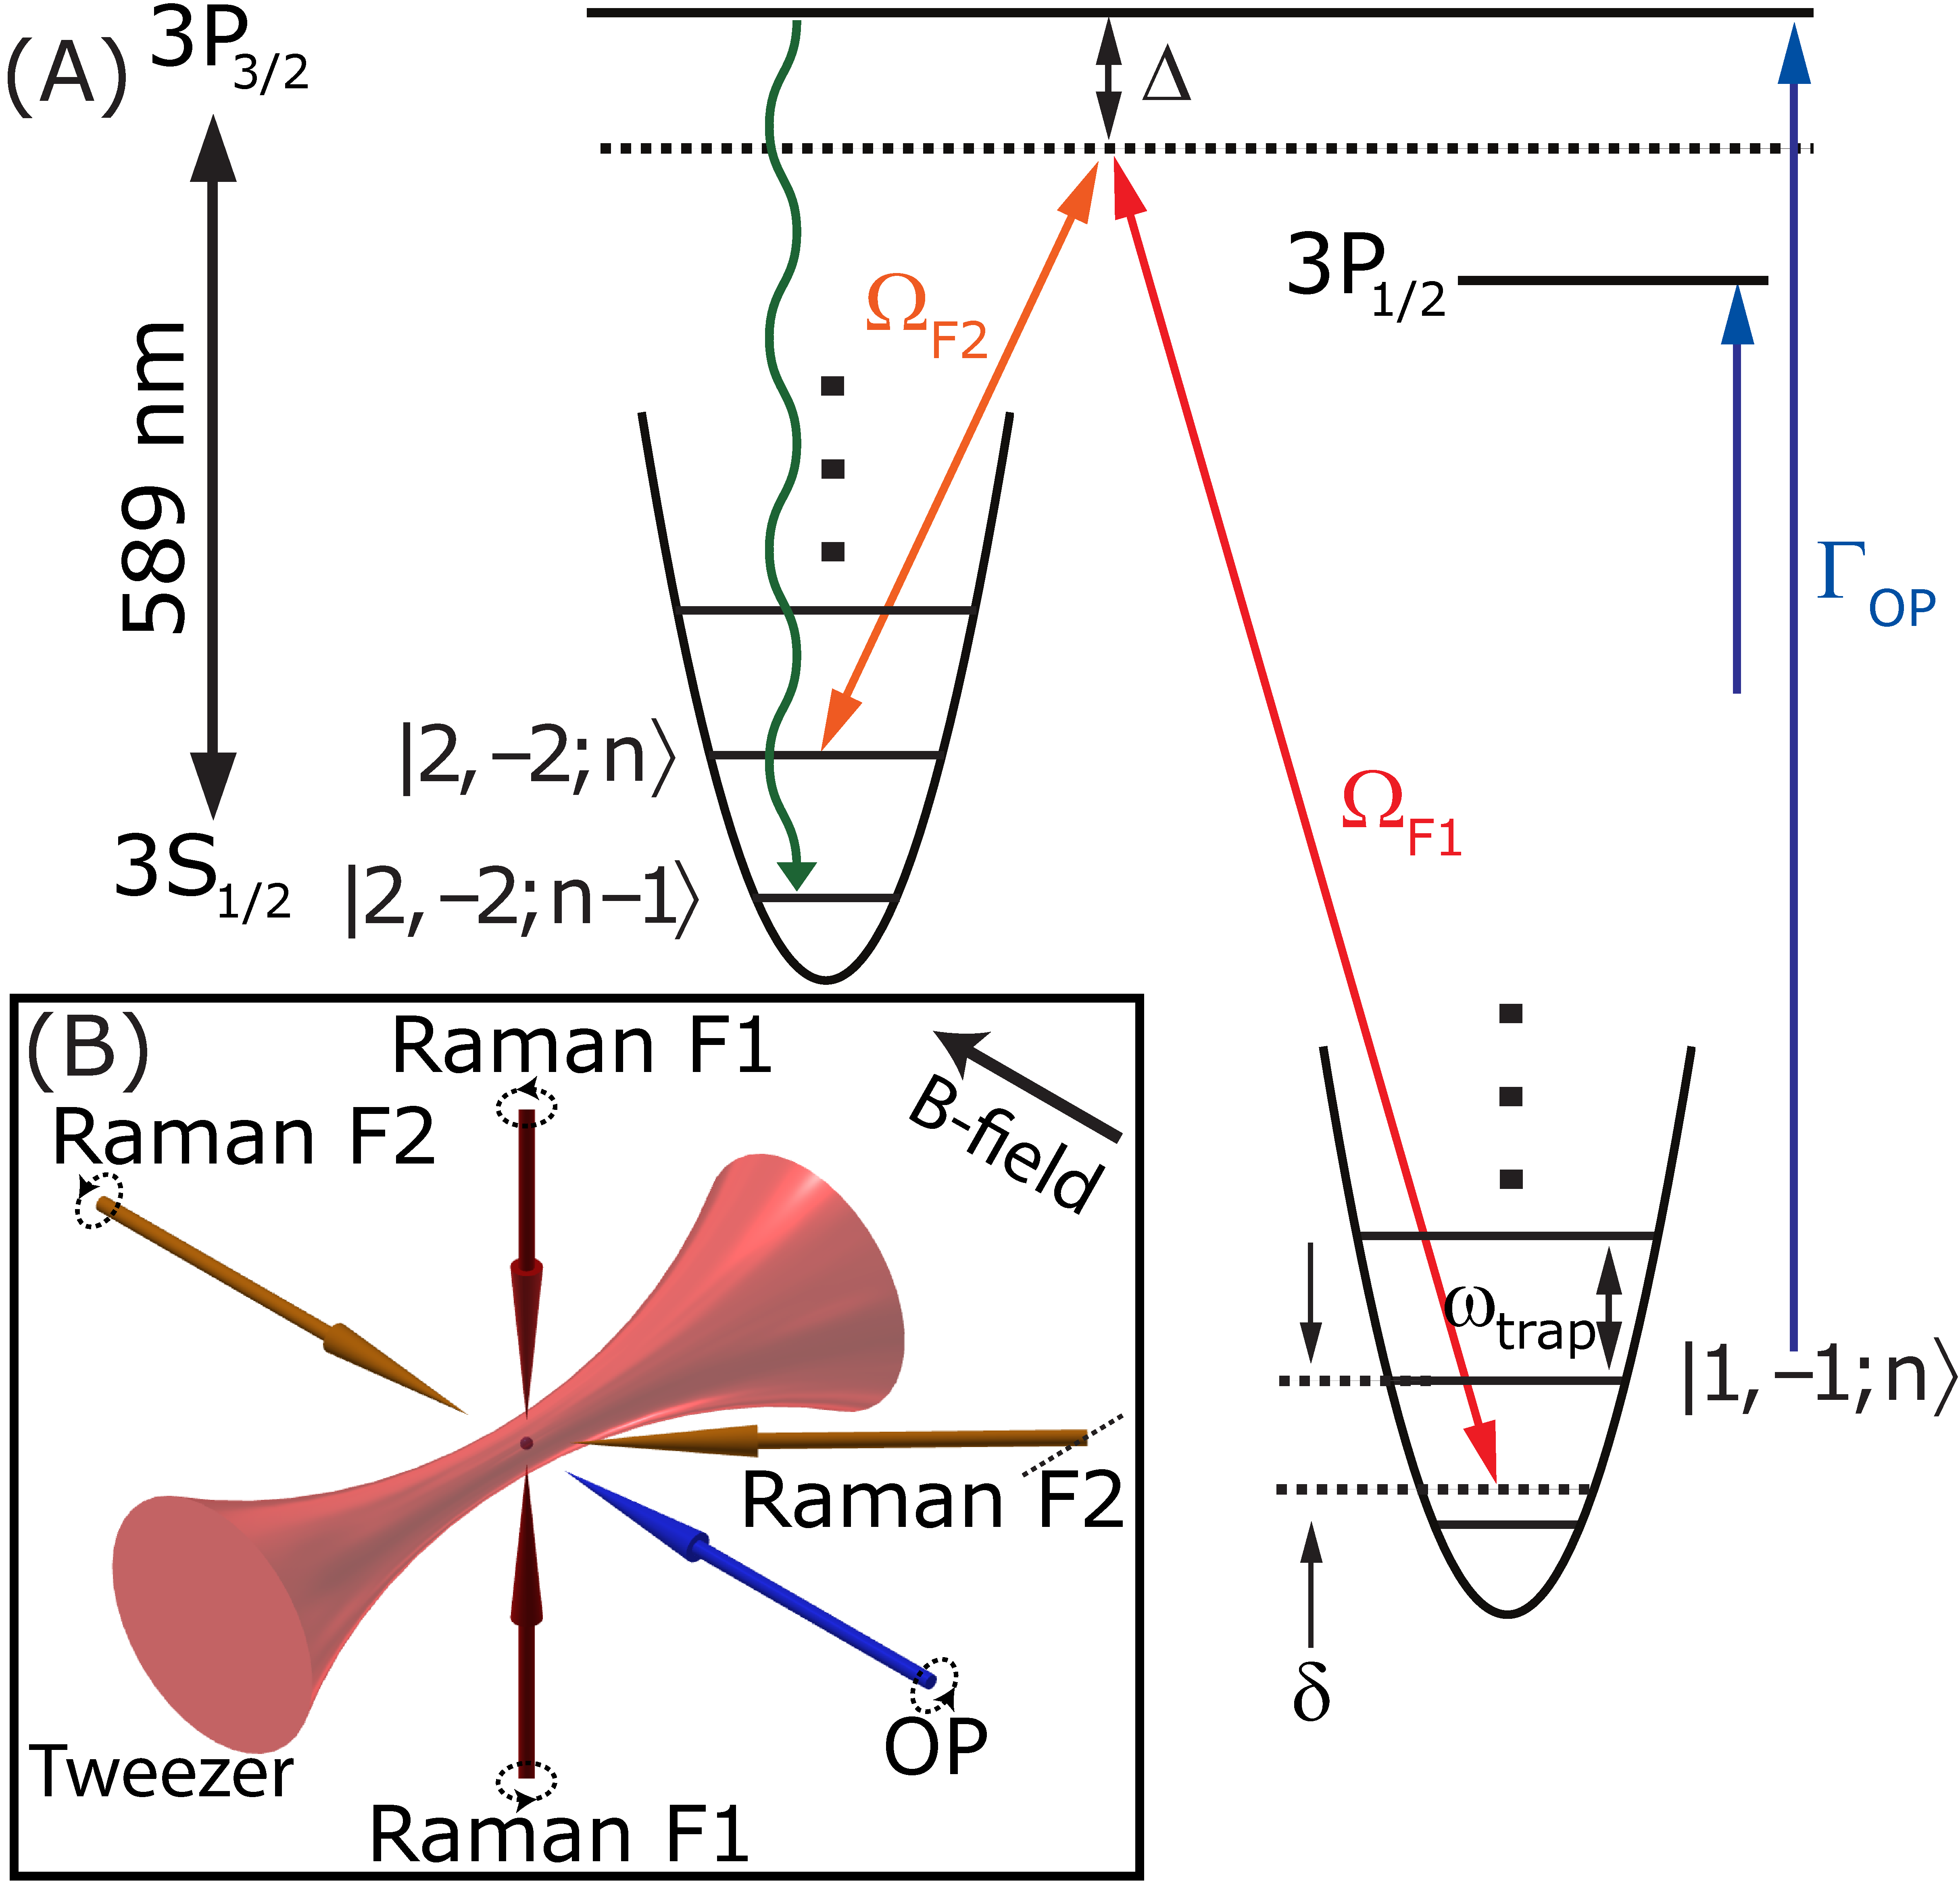
\includegraphics[height=5.2cm]{imgs/Na_RSC_schematic.pdf}
  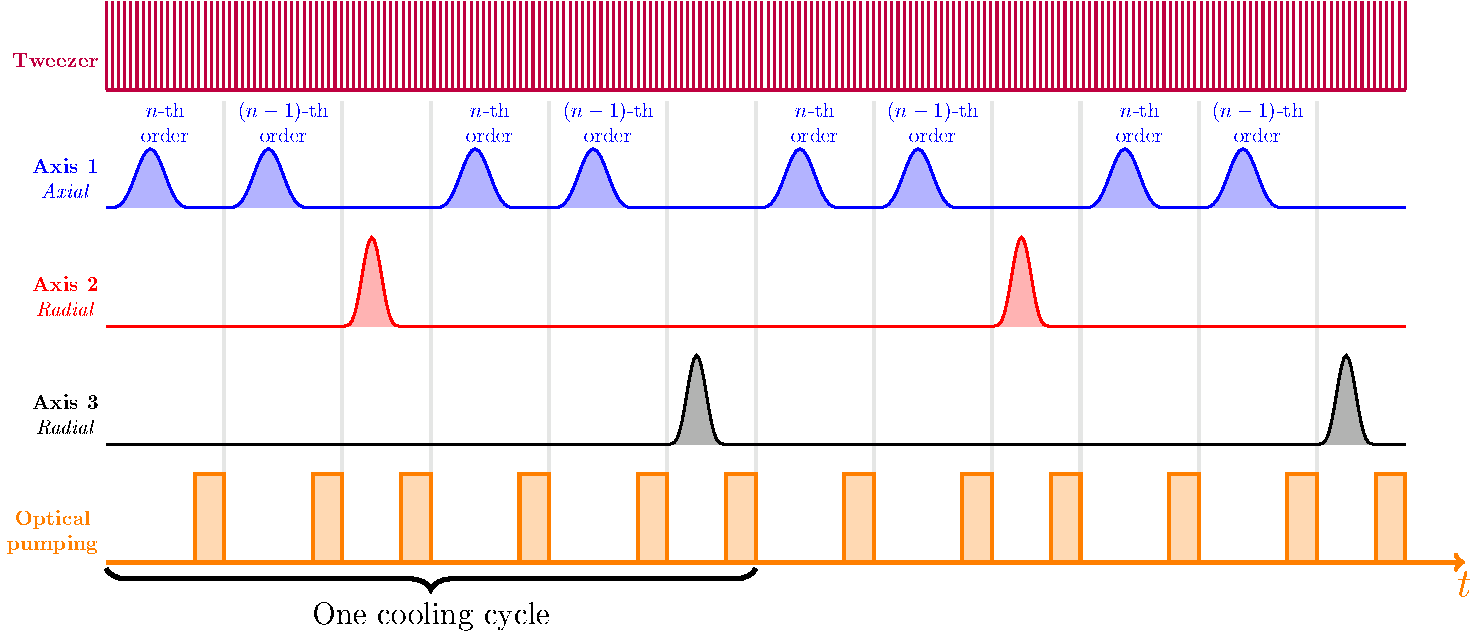
\includegraphics[height=4.5cm]{sequence.pdf}
  \caption{(A) Energy levels and schematic of Raman sideband cooling.
    The Raman transitions have a one photon detuning $\Delta=25$ GHz from the D2 line.
    We use D1 light with $\sigma^-$ polarization to repump atoms out of $|F=2,m_F=-1\rangle$
    state to minimize heating on the atom in $|F=2,m_F=-2\rangle$ state
    (B) Geometry and polarizations of the Raman and optical pumping beams relative to the
    optical tweezer and bias magnetic field.
    (C) Schematic of the cooling sequence. The tweezer switches at 3 MHz to
    reduce light shifts during optical pumping. Each cooling cycle consists of $8$ pulses.
    The four axial pulses are addressing two neighboring cooling orders.
    The two pulses in each radial directions are either addressing two neighboring cooling orders
    or having different length on the first order when most of the population are below $n=3$
    towards then end of the cooling sequence.
    \label{f-setup}}
\end{figure*}
\begin{figure}[b]
  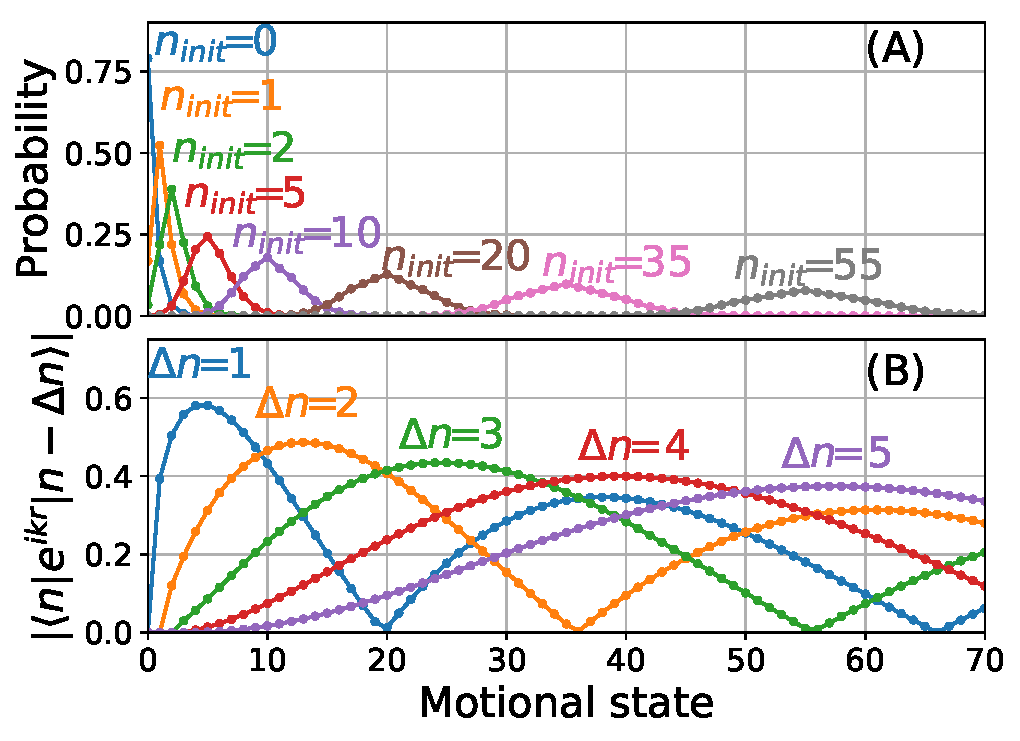
\includegraphics[width=8.5cm]{imgs/fig2_raman_op.pdf}
  \caption{Matrix elements and heating as a function of motional state.
    The range plotted covers $95\%$ of the initial thermal distribution.
    (A) Matrix elements for Raman transition in the axial direction showing deviation from
    $\sqrt{n}$ scaling and multiple minimums for different sideband orders.
    ($k$ is the difference in wave vector of the Raman beams,
    $r$ is the coordinate in axial direction).
    (B) Average change in motional state after the optical pumping step for all three axis.
    Due to the large Lamb-Dicke parameter,
    there is a high probability of $n$ changing especially in the axial direction.
    \label{f-ld}}
\end{figure}
\begin{figure*}
  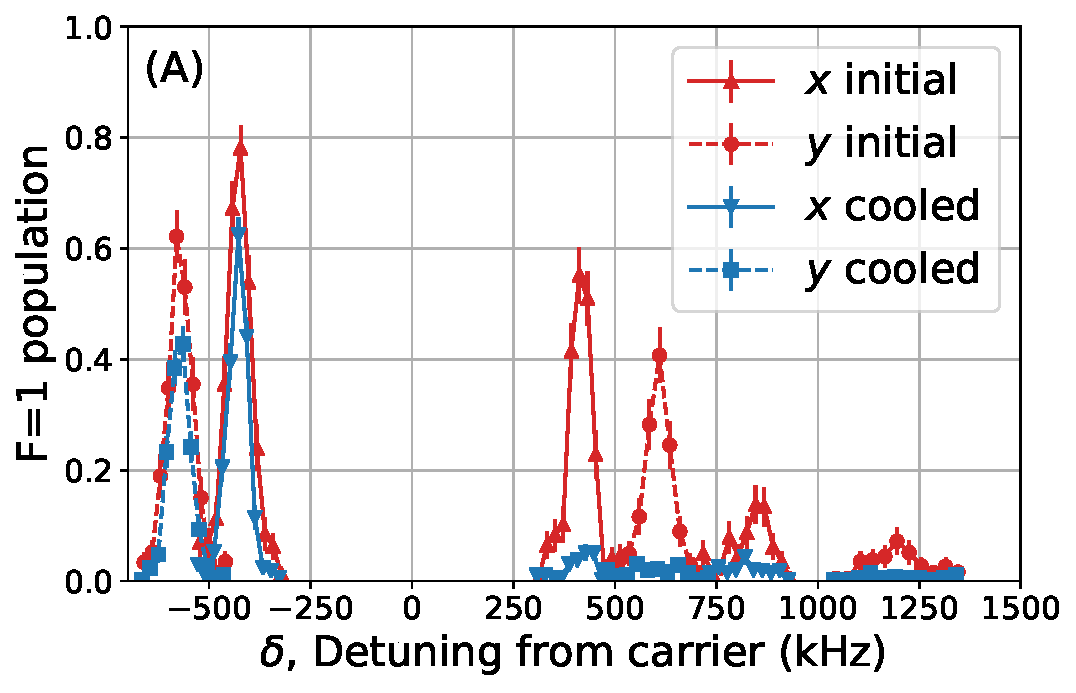
\includegraphics[height=4.2cm]{imgs/spectrum_r.pdf}
  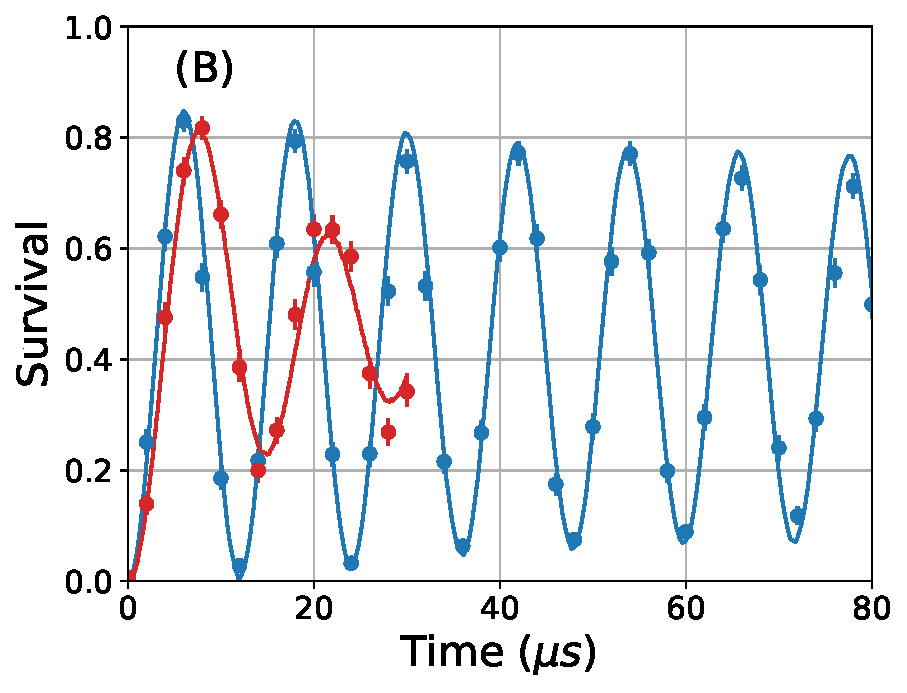
\includegraphics[height=4.2cm]{imgs/rabi_flop_r3_0.pdf}
  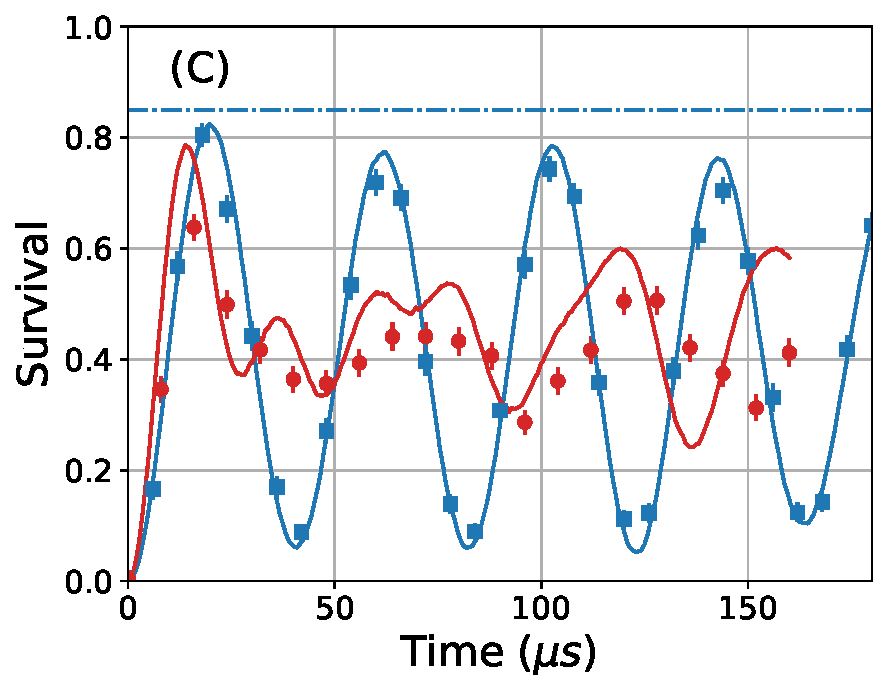
\includegraphics[height=4.2cm]{imgs/rabi_flop_r3_p1.pdf}
  \caption{(A) Radial Raman sideband spectrum of first order heating, first order cooling and
    second order cooling before and after Raman sideband cooling.
    (B,C) Rabi flopping on axis 3 (B) carrier and (C) first order heating sideband
    before (red) and after (blue) cooling.
    Solid lines in (B) and (C) are theoretical calculation of the Rabi flopping.
    The blue lines corresponds to a ground state probability of $93\%$ after cooling and
    the red lines corresponds to a thermal distribution of $70$ $\mu$K before cooling.
    \label{f-radial}}
\end{figure*}
\begin{figure*}
  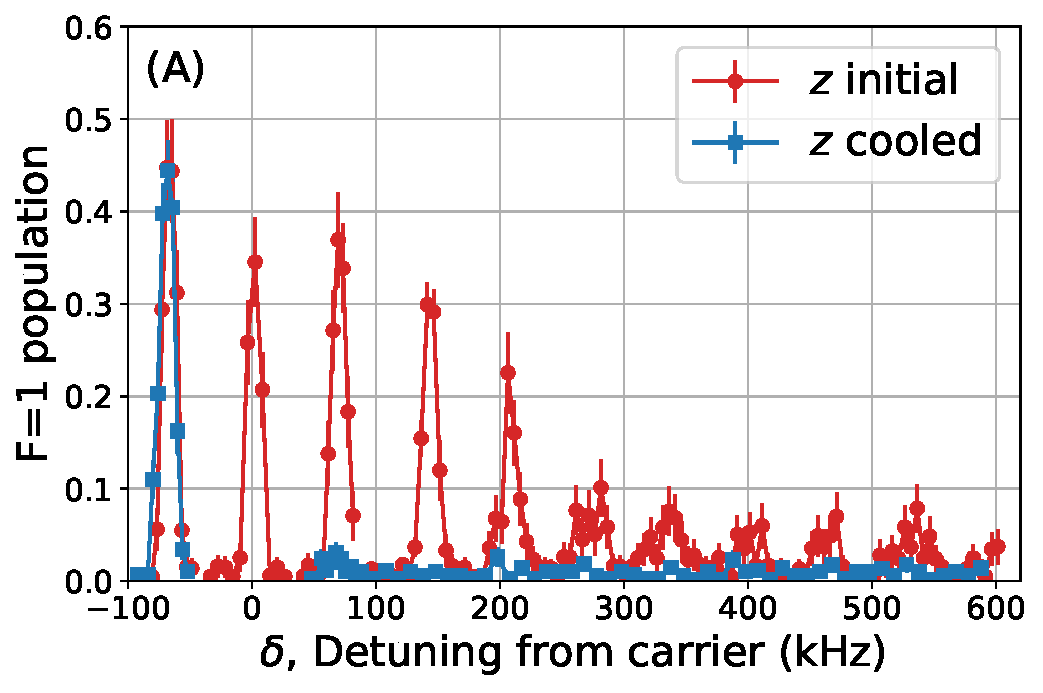
\includegraphics[height=4.2cm]{imgs/spectrum_a1.pdf}
  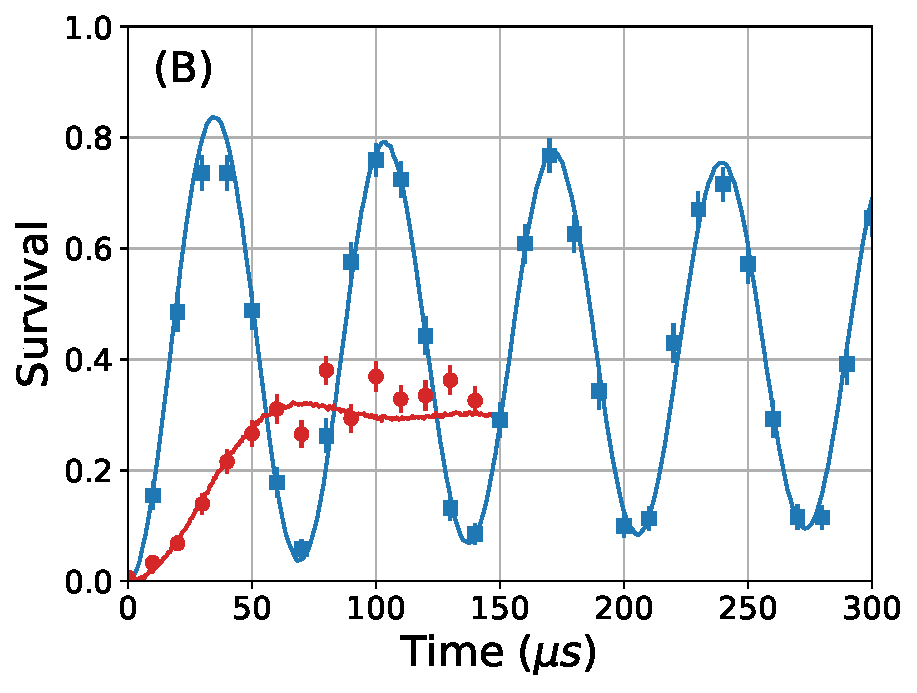
\includegraphics[height=4.2cm]{imgs/rabi_flop_a1_0.pdf}
  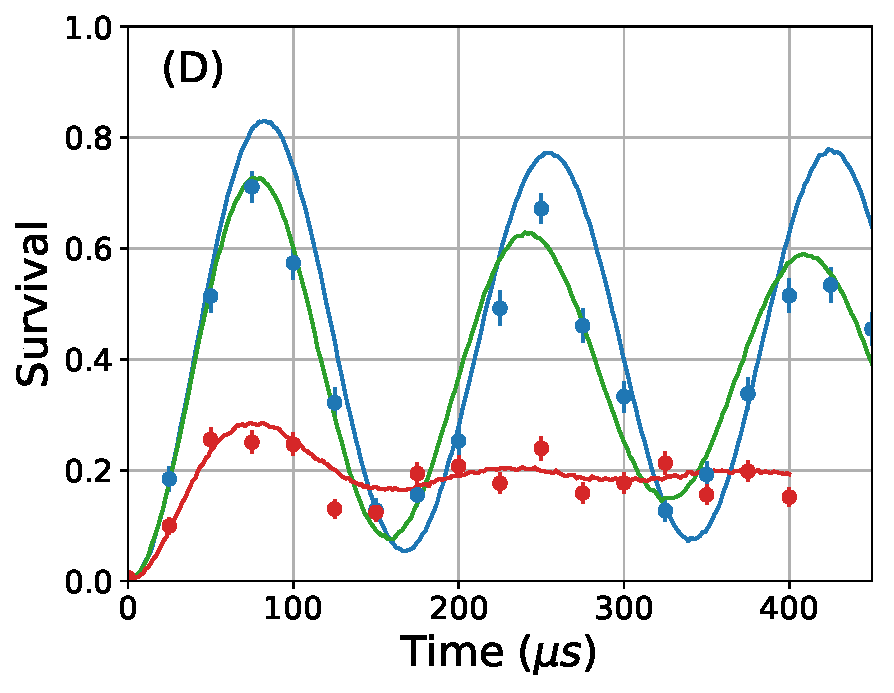
\includegraphics[height=4.2cm]{imgs/rabi_flop_a1_p1.pdf}
  \caption{(A) Axial Raman sideband spectrum from first order heating to eighth order cooling
    before and after Raman sideband cooling.
    The data for the second and higher orders of cooling sidebands are taken with 150 $\mu$s
    pulse time and the rest are taken with 125 $\mu$s pulse time.
    (B,C) Rabi flopping on axial (B) carrier and (C) first order heating sideband
    before (red) and after (blue) cooling.
    Solid lines in (B) and (C) are theoretical calculation of the Rabi flopping.
    The blue and green lines corresponds to a ground state probability of $92\%$ after cooling and
    the red lines corresponds to a thermal distribution of $70$ $\mu$K before cooling.
    The blue lines does not take into account the effect of decoherence due to resonance
    fluctuation. By comparing it to the green line in (C), which includes a $3$ kHz fluctuation,
    we can clearly see that this effect is the strongest for the after cooling data on
    the axial heating sideband where the Rabi frequency is the lowest.
    \label{f-axial}}
\end{figure*}

Bottom-up assemblies of trapped neutral atoms in optical tweezer arrays
are an exciting platform to study quantum information and quantum simulations~\cite{Schlosser2001,Weiss2004,Isenhower2010,Wilk2010,Kaufman2015,Labuhn2016,Murmann2015}.
The inherent single-particle detection and control that combines with tunable interactions
are keys to demonstrate neutral atom based quantum logic gates~\cite{Isenhower2010,Wilk2010},
novel quantum phases~\cite{Labuhn2016}, and single-photon switches~\cite{Dayan2008,Tiecke2014}.
Advances of real-time re-arrangement of optical tweezers enable rapid preparation of atoms
in large and complex geometries with high fidelity~\cite{Barredo2016,Endres2016}.
Adding quantum motional control of individual
atoms~\cite{Li2012,Kaufman2012,Thompson2013,Liu2017,Robens2017} further allows
efficient coupling of single atoms to photonic crystal cavity~\cite{Thompson2013a},
high-fidelity single qubit gates~\cite{Wang2016},
and laser-cooled bosons to exhibit indistinguishability
through Hong-Ou-Mandel interference~\cite{Kaufman2014}.

Extend such an optical tweezer array to polar molecules could open up a large range of
new applications that exploits rich molecular long-lived internal states
and high degrees of tunable interactions~\cite{DeMille2002,Ni2008,Gorshkov2011,Yan2013}.
Molecules could be assembled from atoms directly inside the optical tweezer~\cite{Liu2017}
or to be loaded from magneto-optical traps
(MOTs)~\cite{Barry2014,Truppe2017SubDoppler,Anderegg2017}.
For either approach, preparing constituent atoms or molecules in the lowest motional
quantum state is important for high efficient molecular assembly
and for long coherence times of any realistic quantum applications.

Prepare quantum ground-state for a variety of systems including
single atoms in optical tweezers~\cite{Kaufman2012,Thompson2013,Liu2017,Robens2017}
has been successful using Raman sideband cooling (RSC)~\cite{Monroe1995,Kerman2000,Han2000}.
However, RSC in these systems has all been applied in the Lamb-Dicke regime \fxnote{define}.
A challenging goal is to apply ground-state cooling to system such as atoms with light masses
or laser-cooled polar molecules, that are often outside of the Lamb-Dicke regime.
In this letter, we overcome this challenge and demonstrate cooling of single sodium atoms
that are trapped in optical tweezers to the motional ground state.
We achieve a single atom ground-state probability of $P_0=77(4)\%$ by utilizing cooling of
very high-order sidebands in a carefully optimized cooling sequence.
Our approach is  general and opens up ground-state cooling for other systems.

Our experiment begins by loading a single sodium atom into an optical tweezer from a MOT
for $250$ ms~\cite{Hutzler2017-LightShifts} and repeats at $2.5$ Hz.
The tweezer is created by focusing a $700$nm laser beam through an NA=$0.55$ objective to
a beam waist of $0.7$ $\mu$m\fxnote{?}.
With $45$mW of tweezer power, the trapping frequencies are
$\{\omega_1,\omega_2,\omega_3\}/2\pi = \{69(1), 430(4), 590(5)\}\ \text{\text{kHz}}$.
Upon loading, an image is taken for $1.5$ms to determine its success.
The same imaging light is used for polarization gradient cooling (PGC) and
reduces the temperature of the single atom to $70$ $\mu$K,
which corresponds to an initial motional state along the three different axes of
$\{\bar n_1, \bar n_2, \bar n_3\}=\{21(2),\, 3.4(2),\, 2.5(2)\}$ (initial $P_0=0.3\%$) in the trap.
A beam with $\sigma^-$-polarization is used to optical pump the atom into
the $|F=2, m_F=-2\rangle$ stretch state.
The hyperfine state detection is done by pushing out atoms in the stretch state with a strong
beam on resonance with the $|F=2, m_F=-2\rangle$ to $|F'=3, m_{F'}=-3\rangle$ transition before
taking the second image.
The state preparation and detection have a combined fidelity of larger than $99$\%.

To further reduce the temperature of the single atom and
to achieve high ground-state preparation fidelity, we apply Raman sideband cooling.
The relevant energy levels, the cooling sequence, and the Raman beam geometries our system
is shown in Figure \ref{f-setup}. Overall, the RSC consists of two steps:
a step to drive a coherent Raman transition while removing motional quanta and
a step to reset the atom internal state via optical pumping (OP).
RSC is applied repeatedly until motional ground state is achieved.

Specifically, Raman transitions are driven in Na between the hyperfine states
$|F=2, m_F=-2\rangle$ and  $|F=1, m_F=-1\rangle$ in the presence of a $8.8$ G magnetic field.
Subsequently, an OP/repump pulse brings the atom back to $|F=2, m_F=-2\rangle$
via spontaneous emissions.
Because any photon scattering is a heating source,
we use a $\sigma^-$-polarized laser resonant with the D1 line for repump,
which is dark to $|F=2, m_F=-2\rangle$ \fxnote{cite ion and K39}.
Compared to using a D2 repump beam, we find a reduction in the $|F=2, m_F=-2\rangle$
scattering rate of a factor of $130(20)$.

For an atom in the motional level $n$, the OP could result in motional-state redistribution
as shown in Fig.~\ref{f-ld}\fxnote{A or B?}. The state redistribution probability,
and hence overall heating, is approximately proportional to the effective Lamb-Dicke parameter
$\eta^{OP}_{\eff}=\sqrt{2n+1}\eta^{OP}$, where $\eta^{OP}=k z_0=k \sqrt{\hbar/2m\omega}$,
$k$ is the optical pumping wavenumber, $z_0$ is the zero-point wavefunction spread,
$m$ is the mass of the atom, and $\hbar$ is the reduced Planck constant.
Such heating presents a major challenge for efficient cooling of single Na atoms
which feature a light mass and short D-line wavelengths.
For our trap frequencies and beam geometry,
$\{\eta^{OP}_1,\eta^{OP}_2,\eta^{OP}_3\} = \{0.602(5), 0.241(2), 0.206(1)\}$.
Combined with a relatively large PGC temperature gives initial
$\{\eta^{OP}_{1\eff},\eta^{OP}_{2\eff},\eta^{OP}_{3\eff}\} = \{4.0(1), 0.67(2), 0.50(1)\}$.
For the weak axial direction, $(\eta^{OP}_{1\eff})^2>1$ is far outside of the Lamb-Dicke regime.
As a result, the average change of motional state per OP step is large,
which creates a large uncertainty on the motional state at the end of a full RSC step.
Scenarios of runaway OP heating from RSC cycles are possible.
As a comparison, the averaged change in motional states over the initial distribution
is $2.4$ in the axial direction, which is significantly greater than $0.89-0.95$
in previous experiments of RSC of Rb and Cs~\cite{Li2012,Kaufman2012,Thompson2013,Liu2017}.

Fortunately, the large Lamb-Dicke parameters also provide a way to overcome OP heating.
The Raman transitions in our configuration have
$\{\eta^R_{1},\eta^R_{2},\eta^R_{3}\} = \{0.40(1), 0.341(2), 0.291(1)\}$,
which allow strong coupling to higher order sidebands for atoms in large motional states
as calculated in Figure~\ref{f-ld}\fxnote{A or B?}.x
To offset heating from OP initially, higher-order Raman cooling sidebands can be utilized
to remove more motional quanta in a single cooling pulse.
Since the coupling strengths of different orders do not reach minima for the same pulse duration,
using multiple orders of cooling sidebands would avoid accumulations of population
near the coupling minima.

Taking the large motional-state changing heating and cooling sources into account,
it was not immediately clear that efficient cooling can be achieved.
We therefore use a Monte-Carlo simulation to guide our search and
to find a robust cooling sequence\footnote{See supplemental material}.
In the simulation, we indeed observe a high heating rate due to the large Lamb-Dicke parameters
and confirm that cooling with higher-order Raman sidebands can suppress heating.
In particular, we find that instead of cooling on only one sideband order repeatedly,
it is more efficient to alternate the cooling pulses (Fig.~\ref{f-setup}C) between two
neighboring orders for the axial direction and 2nd- and 1st-orders for the radial directions
to minimize the accumulation of the atom in motional states that have zero Raman coupling.
The simulation also indicates setting the coupling strength of each cooling sideband
to drive a Rabi $\pi$ pulse corresponding to the maximum matrix element motional state
(i.e. the maxima in \ref{f-ld}\fxnote{A or B?}).
Such choice insures each order cools a range of states that have the strongest
couplings and leaves other sidebands to cool the rest.
The efficiency of cooling on higher-order sidebands diminishes
as the atom approaches the ground state.
Therefore, the final cooling cycles utilize only the first-order sideband
while alternating between different axes.

Guided by the promising simulation results,
we construct our axial cooling sequence by starting at the highest
two observed cooling sidebands (8th- and 7th-orders)
and decreasing the orders after $6$ to $15$ cycles.
This process is repeated until we reach the first order cooling sideband where most of the
population are in the first few excited state at which point we switch to only cooling on the
first order sideband with two different pulse lengths in order to efficiently cool atoms in the
few remaining motional states.
The radial cooling is done similarly to the axial cooling with the initial cooling orders being
the 2nd and 1st order and switching to first order only after $20$ to $30$ pulses.
This sequence gives good initial cooling performance which is used to measure experimental
parameters, including the Rabi rates of the Raman beams and optical pumping rates,
in order to optimize the sequence further.

Two additional challenges of cooling single sodium atoms are
further identified and addressed experimentally.
First, the high initial temperature causes population in high motional states
means that the atoms sample anharmonicity of the trap away from the center.
In order to address trap anharmonicity, we drive sidebands with a large Rabi frequency
and short pulses to Fourier broaden spectrum coverage.
For the higher trap frequency radial directions, anharmonicity is calculated to be 1kHz/n,
Rabi frequency of at least $15$ kHz is needed to couple to $99$\% population up to $n=15$.
Second, the  tweezer trap  causes a large AC Stark shift (as large as $300$ MHz)
in the excited state. This creates  a large, position-dependent OP detuning
and mixes the excited-state hyperfine levels, and therefore reduces the optical pumping fidelity.
We solve this issue by switching the trapping light at 3 MHz during the whole cooling sequence,
similar to our loading and imaging process~\cite{Hutzler2017-LightShifts},
while leaving OP on with constant intensity.
Due to the large light shift, the optical pumping is effectively off when the trap light is on.
Since the atom can only be addressed by the optical pumping light when the trap light is off,
the effect of light shift on optical pumping fidelity is suppressed.

Our final cooling results are shown in Fig.~\ref{f-radial} and \ref{f-axial}.
In total, $1000$ cooling pulses (for $100$ ms) are applied along three axes with
cooling begins on the radial second order to remove most energy initially.
To characterize the single atom thermal occupation before and after cooling,
we perform Raman sideband thermometry before and after cooling\fxnote{add citation?}.
For the more tightly confined radial directions (non-degenerate),
we observe clear first-order heating, first-order cooling,
and second-order cooling sidebands before RSC as is shown in red in Figure \ref{f-radial}A.

After cooling, the first and second order cooling sidebands on both radial axes are suppressed.
It is important to note that the simple sideband thermometry formula,
which predicts the ratio of the cooling and heating sideband heights to be $\bar n / (\bar n + 1)$,
assumes that the coupling strength for different motional states to be proportional to $\sqrt{n}$.
Outside of the Lamb-Dickes regime, however,
the coupling strength deviates from this simple scaling rule rapidly
as shown in figure \ref{f-ld}A and since the Raman spectroscopy is performed
with a relatively large Raman Lamb-Dickes parameters $\eta^R$, we cannot use this formula to
measure $\bar n$. Instead, given the absence of the second order cooling sideband,
we assume that the atoms are colder than

\fxnote{How is the thermometry done? pulse duration etc.}
, we perform sideband thermometry
by taking the ratio of the peaks of first-order cooling and heating sidebands to measure $\bar n / (\bar n + 1)$ \fxnote{cite}.
We found $\{\bar n =,\bar n =\}$, which corresponds to a ground state population of $90(2)\%$
and $94(3)\%$ along the two radial directions.

we therefore use an independent measurement of Rabi flopping on the carrier (Fig. \ref{f-radial}B)
and first-order heating(Fig. \ref{f-radial}C) sidebands
to verify the ground-state population~\cite{Meekhof1996}.
The data is fitted using the same Monte-Carlo simulation we used to simulate the cooling
which yields $89(2)\%$ and $92(2)\%$ and show good agreement with
the population extracted from the sideband thermometry.
We also extracted the initial temperature before cooling
from the motional-state decohered Rabi flopping and obtained \fxnote{70(?)} $\mu$K.

For the weaker axial direction, cooling is much more challenging
due to the large $\eta^{OP}_{eff1}\approx 4.0(2)$.
In the Raman sideband thermometry, we observe up to 8th-order cooling sidebands initially,
which indicates population in highly-excited motional states.
Nevertheless, our cooling sequence works efficiently as all the cooling sidebands are suppressed
after RSC (Fig.~\ref{f-axial}).
The ground-state probability calculated using the ratio of first-order sideband heights yields
$92(3)\%$. We also perform Rabi flopping on the carrier(Figure~\ref{f-axial}B)
and extracted a ground-state population of \fxnote{??}\%, in agreement with the other method.
For the first-order heating sideband Rabi flopping (Figure~\ref{f-axial}C),
we observed additional decoherence that is more produced due to the slower Rabi frequency.
The decoherence time scale is consistent with magnetic field fluctuations of $1.5$ mG
that we measure independently in the lab, which produces a Zeeman shift of $\sim 3$ kHz.

Combining the axial and radial cooling results,
we have prepared a single Na atom with 3D ground state probability of $77(4)\%$.
We measuring a heating rate of the single atoms in the tweezer to be \fxnote{??}\%
due to trapping light scattering.\fxnote{ciet Grimm}
The ground-state preparation fidelity is currently limited by off-resonant scattering
from the Raman beams,
which are measured to be between $3$ to $15$ kHz for the detuning and power we use,
and the resonance shift caused by magnetic field fluctuations.
In addition, there are $15$\% population loss during the experiment,
including $5\%$ from single atom imaging and  $10\%$ very high-lying initial motional states
that are not efficiently cooled by RSC, but off-resonantly heat by the Raman beams.
We are planing to improve these by increasing the detuning of the Raman beams,
addressing wider range of anharmonicity by frequency sweep...,
implementing better control of the magnetic field and optimize the temperature during imaging.
We expect these changes to improve the cooling performance further.
Another improvement could be to implement grey molasses cooling to achieve
a lower starting temperature before RSC. \fxnote{cite}

We have shown that despite the difficulty in achieving a low optical cooling temperature
of light mass sodium atoms, reliable three dimensional cooling
with significant ground-state population can be achieved by using high-order Raman sidebands
in an optimized cooling sequence in the presence of temporal switching tweezer trap.
These techniques are well-suited for a large variety of systems
and open up a route to ground-state cooling to other species including molecules and exotic atoms.

We thank T. Rosenband and J. Hood for discussion.
This work is supported by the NSF through the Harvard-MIT CUA,
the AFOSR Young Investigator Program, the Arnold and Mabel Beckman Foundation,
and the Alfred P. Sloan Foundation.

% Missing:
% ?? Blackman pulse vs square pulse

\bibliography{paper}
\end{document}
